\subsection{Sprint One}
\begin{frame}
\frametitle{Sprint One}
\begin{center}
\begin{columns}
\begin{column}{0.35\textwidth}
\only<2,3>{\quad Bug fixing\\ \quad\includegraphics[height=1.5cm]{images/bugfixing}}
\end{column}
\begin{column}{0.5\textwidth}
\only<1>{\quad Bug fixing\\ \includegraphics[height=4cm]{images/bugfixing}}
\only<2>{\quad Improve Drawer\\ 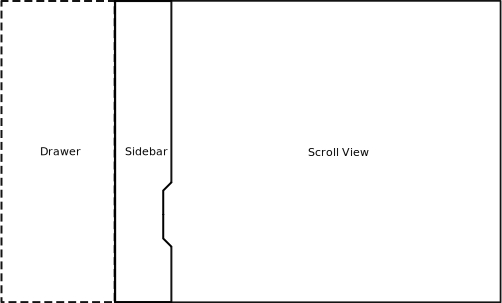
\includegraphics[height=4cm]{images/drawer}}
\only<3>{\quad Functional Testing\\\includegraphics[height=4cm]{images/test}}
\end{column}
\begin{column}{0.25\textwidth}
\only<3>{Improve Drawer\\ 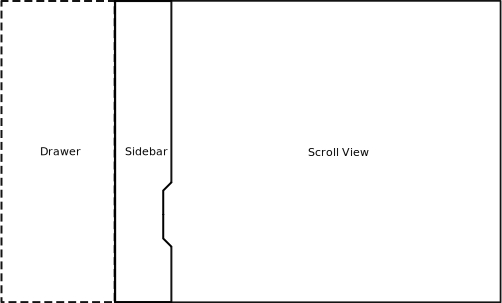
\includegraphics[height=1.5cm]{images/drawer}}
\end{column}
\end{columns}
\end{center}
\end{frame}

\begin{frame}
\frametitle{Sprint One}

Product Demonstration
\begin{itemize}
\item Developments after Sprint One
\end{itemize}


\end{frame}

\subsection{Sprint Two}
\begin{frame}
\frametitle{Sprint Two}
\centering
\begin{itemize}
\item<1>Create Prototypes of Settings
\item<2>Customer meetings
\end{itemize}
\only<1>{ \includegraphics[height=4cm]{images/prototype}}
\only<2>{\includegraphics[height=4cm]{images/customer}}
\end{frame}

\subsection{Sprint Three}
\begin{frame}
\frametitle{Sprint Three}
\begin{center}
\textbf{Implementation of Settings:}
\end{center}
\begin{columns}
\begin{column}{0.5\textwidth}

          \begin{center}
\only<2,3,4,5>{Settings for Launcher\\
           	 \includegraphics[height=2cm]{images/giraf}}
        \end{center}
        \begin{center}
       		\only<3,4,5>{Application Management\\
             \includegraphics[height=2cm]{images/apps}}
        \end{center}
\end{column}
\begin{column}{0.5\textwidth}
        \begin{center}
               		\only<4,5>{Stemmespillet\\
                     \includegraphics[height=2cm]{../report/figures/pres/settingscars}}
         \end{center}
        \begin{center}
                    \only<5> {Sekvens\\
                     \includegraphics[height=2cm]{../report/figures/pres/settingssekvens}}
        \end{center}
\end{column}
\end{columns}
\end{frame}

\subsection{Sprint Four}
\begin{frame}
\frametitle{Sprint Four}
\begin{center}
Instant Data Analysis\\
\begin{columns}
\begin{column}{0.5\textwidth}
\includegraphics[height=3cm]{images/usertest}
\end{column}
\begin{column}{0.5\textwidth}

\begin{description}
\item<1>[Strengths:] Quick, easy and efficient
\item<2>[Weaknesses:] Not all errors are caught
\end{description}

\end{column}
\end{columns}
\end{center}
\end{frame}
\subsection{Sprint Four}
\begin{frame}
\frametitle{Sprint Four}
\begin{center}
Instant Data Analysis\\
\begin{columns}
\begin{column}{0.5\textwidth}
\includegraphics[height=3cm]{images/usertest}
\end{column}
\begin{column}{0.5\textwidth}

\only<1,2,3>{\textbf{Results:}}
\begin{itemize}
\item<1>Names of tabs
\item<2>Marking Apps
\item<3>Overall Positive
\end{itemize}

\end{column}
\end{columns}
\end{center}
\end{frame}

\begin{frame}

\frametitle{Sprint Four}
\begin{center}
Final Product Demonstration
\end{center}
\end{frame}